\documentclass{article}
\usepackage{graphicx}
\usepackage{amssymb}
\usepackage{amsmath}
\usepackage{float}

\usepackage[margin=1in]{geometry}


\begin{document}



\title{16-720 Computer Vision: Homework 5}
\author{Xiang Zhi Tan}

\maketitle
\subsection*{Q1.0}
$(M - w) \times (N - h)$ windows

\subsection*{Q1.2}
When it is a mission critical application where the application cannot tolerate even single error on true positive even if it's not able to detect all the true positive. For instance, a spam filter would like to have a high precision even if the recall isn't high because it's better to misclassifyi a spam as a normal email than a normal email as a spam. Here's one example of that. Let say there are 10 emails, the program classifies 4 of them as spams which all are correct, whereas the emails that are classified as normal emails, 4 of them are spams. The precision rate would be 4/4, where as recall rate is 4/8. Here the normal accuracy would be 6/10. In this case, the normal accuracy is actually lower compare to the precision rate. Even thought, the general accuracy is lower, the important part is that none of the normal email was accidentally classified as spam which would cause a lot of inconvenience to the user.

\subsection*{Q1.3}
1 exmplar detectors. Again one template detector.
% \begin{figure}[H]
%     \centering
%     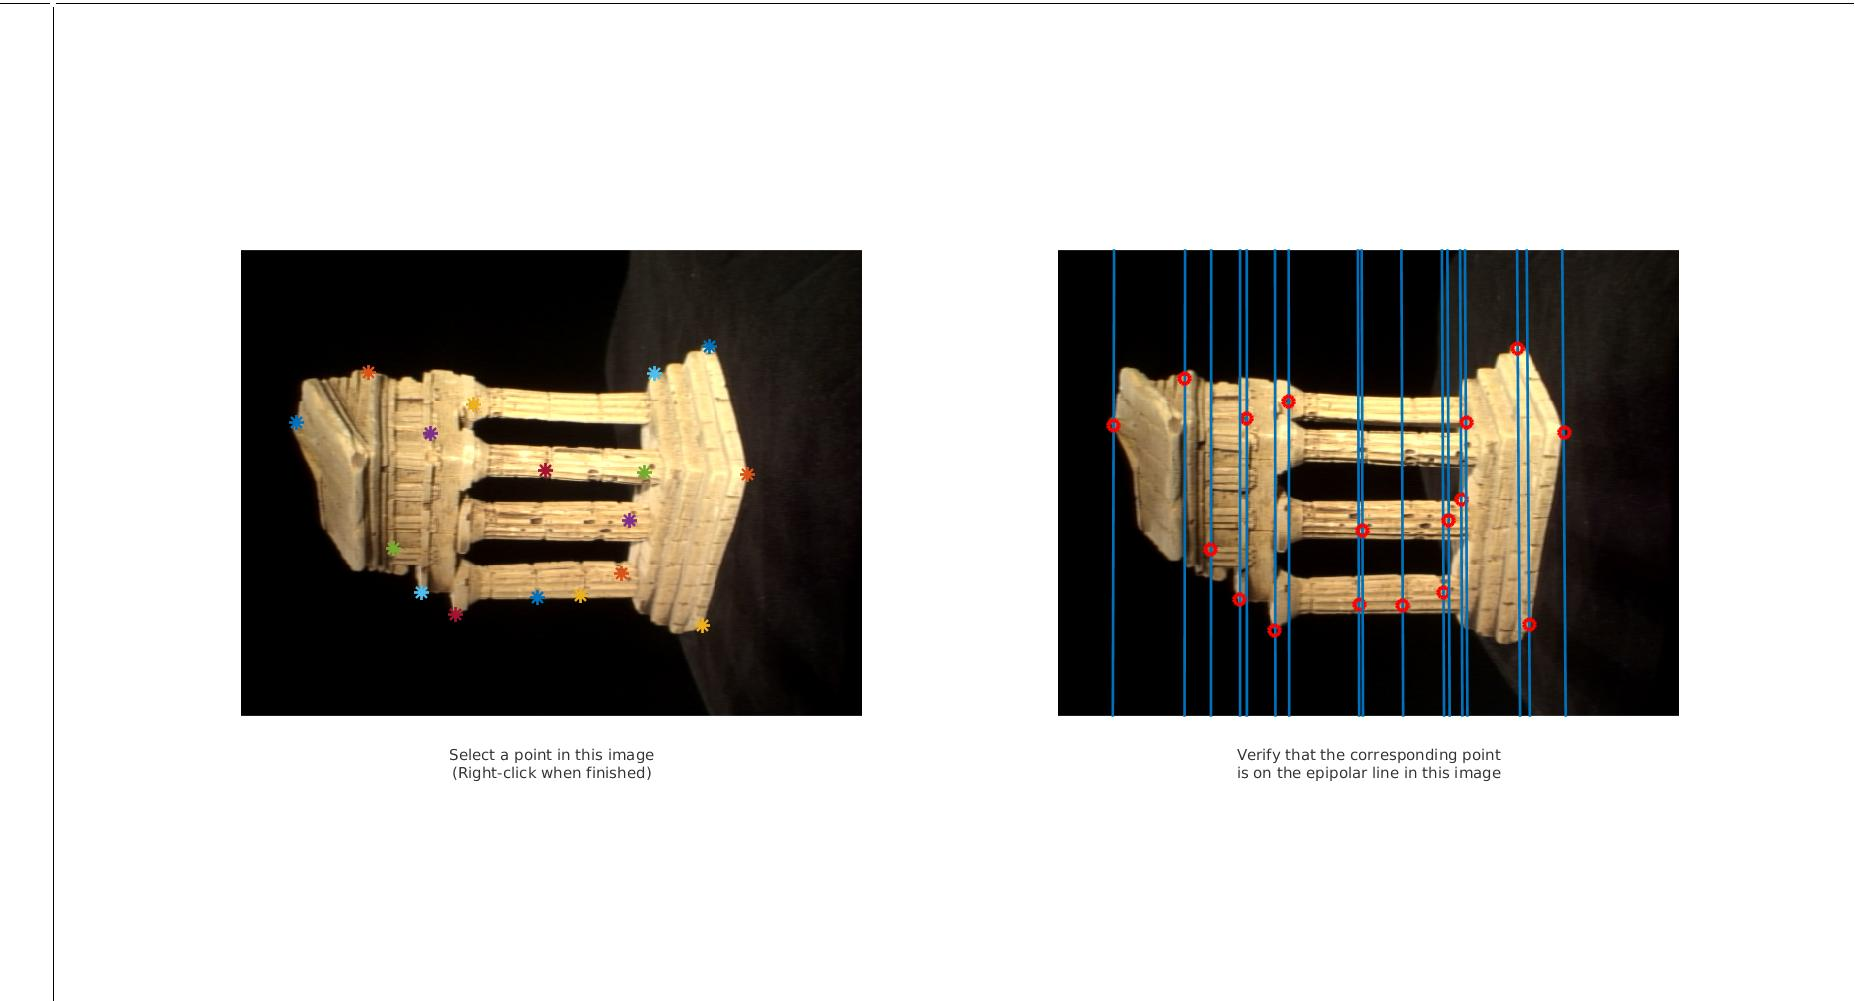
\includegraphics[width=6.5in]{./figures/q2_6}
% \end{figure}
\end{document}